%%%%%%%%%%%%%%%%%%%%%%%%%%%%%%%%%%%%%%%%%
% Masters/Doctoral Thesis 
% LaTeX Template
% Version 2.5 (27/8/17)
%
% This template was downloaded from:
% http://www.LaTeXTemplates.com
%
% Version 2.x major modifications by:
% Vel (vel@latextemplates.com)
%
% This template is based on a template by:
% Steve Gunn (http://users.ecs.soton.ac.uk/srg/softwaretools/document/templates/)
% Sunil Patel (http://www.sunilpatel.co.uk/thesis-template/)
%
% Template license:
% CC BY-NC-SA 3.0 (http://creativecommons.org/licenses/by-nc-sa/3.0/)
%
%%%%%%%%%%%%%%%%%%%%%%%%%%%%%%%%%%%%%%%%%

%----------------------------------------------------------------------------------------
%	PACKAGES AND OTHER DOCUMENT CONFIGURATIONS
%----------------------------------------------------------------------------------------

\documentclass[
11pt, % The default document font size, options: 10pt, 11pt, 12pt
%oneside, % Two side (alternating margins) for binding by default, uncomment to switch to one side
english, % ngerman for German
singlespacing, % Single line spacing, alternatives: onehalfspacing or doublespacing
%draft, % Uncomment to enable draft mode (no pictures, no links, overfull hboxes indicated)
%nolistspacing, % If the document is onehalfspacing or doublespacing, uncomment this to set spacing in lists to single
%liststotoc, % Uncomment to add the list of figures/tables/etc to the table of contents
%toctotoc, % Uncomment to add the main table of contents to the table of contents
%parskip, % Uncomment to add space between paragraphs
%nohyperref, % Uncomment to not load the hyperref package
headsepline, % Uncomment to get a line under the header
%chapterinoneline, % Uncomment to place the chapter title next to the number on one line
%consistentlayout, % Uncomment to change the layout of the declaration, abstract and acknowledgements pages to match the default layout
openany
]{MastersDoctoralThesis} % The class file specifying the document structure

\usepackage[utf8]{inputenc} % Required for inputting international characters
\usepackage[T1]{fontenc} % Output font encoding for international characters

\usepackage{mathpazo} % Use the Palatino font by default

\usepackage[backend=bibtex,style=authoryear,natbib=true]{biblatex} % Use the bibtex backend with the authoryear citation style (which resembles APA)

\addbibresource{example.bib} % The filename of the bibliography

\usepackage[autostyle=true]{csquotes} % Required to generate language-dependent quotes in the bibliography

%----------------------------------------------------------------------------------------
%	MARGIN SETTINGS
%----------------------------------------------------------------------------------------

\geometry{
	paper=a4paper, % Change to letterpaper for US letter
	inner=2.5cm, % Inner margin
	outer=3.8cm, % Outer margin
	bindingoffset=.5cm, % Binding offset
	top=1.5cm, % Top margin
	bottom=1.5cm, % Bottom margin
	%showframe, % Uncomment to show how the type block is set on the page
}

%----------------------------------------------------------------------------------------
%	THESIS INFORMATION
%----------------------------------------------------------------------------------------

\thesistitle{Neural architecture search: a probabilistic approach} % Your thesis title, this is used in the title and abstract, print it elsewhere with \ttitle
\supervisor{Yuriy \textsc{Khoma}} % Your supervisor's name, this is used in the title page, print it elsewhere with \supname
\examiner{} % Your examiner's name, this is not currently used anywhere in the template, print it elsewhere with \examname
\degree{Master of Science} % Your degree name, this is used in the title page and abstract, print it elsewhere with \degreename
\author{Volodymyr \textsc{Lut}} % Your name, this is used in the title page and abstract, print it elsewhere with \authorname
\addresses{} % Your address, this is not currently used anywhere in the template, print it elsewhere with \addressname

\subject{Data Science} % Your subject area, this is not currently used anywhere in the template, print it elsewhere with \subjectname
\keywords{} % Keywords for your thesis, this is not currently used anywhere in the template, print it elsewhere with \keywordnames
\university{\href{http://www.ucu.edu.ua}{Ukrainian Catholic University}} % Your university's name and URL, this is used in the title page and abstract, print it elsewhere with \univname
\department{\href{http://department.university.com}{Faculty of Applied Sciences}} % Your department's name and URL, this is used in the title page and abstract, print it elsewhere with \deptname
\group{\href{http://researchgroup.university.com}{Department of Computer Sciences}} % Your research group's name and URL, this is used in the title page, print it elsewhere with \groupname
\faculty{\href{http://faculty.university.com}{}} % Your faculty's name and URL, this is used in the title page and abstract, print it elsewhere with \facname

\AtBeginDocument{
\hypersetup{pdftitle=\ttitle} % Set the PDF's title to your title
\hypersetup{pdfauthor=\authorname} % Set the PDF's author to your name
\hypersetup{pdfkeywords=\keywordnames} % Set the PDF's keywords to your keywords
}

\begin{document}
\frontmatter % Use roman page numbering style (i, ii, iii, iv...) for the pre-content pages

\pagestyle{plain} % Default to the plain heading style until the thesis style is called for the body content

%----------------------------------------------------------------------------------------
%	TITLE PAGE
%----------------------------------------------------------------------------------------

\begin{titlepage}
\begin{center}

\vspace*{.06\textheight}
{\scshape\LARGE \univname\par}\vspace{1.5cm} % University name
\textsc{\Large Master Thesis}\\[0.5cm] % Thesis type

\HRule \\[0.4cm] % Horizontal line
{\huge \bfseries \ttitle\par}\vspace{0.4cm} % Thesis title
\HRule \\[1.5cm] % Horizontal line
 
\begin{minipage}[t]{0.4\textwidth}
\begin{flushleft} \large
\emph{Author:}\\
\href{http://www.johnsmith.com}{\authorname} % Author name - remove the \href bracket to remove the link
\end{flushleft}
\end{minipage}
\begin{minipage}[t]{0.4\textwidth}
\begin{flushright} \large
\emph{Supervisor:} \\
\href{http://www.jamessmith.com}{\supname} % Supervisor name - remove the \href bracket to remove the link  
\end{flushright}
\end{minipage}\\[3cm]
 
\vfill

\large \textit{A thesis submitted in fulfillment of the requirements\\ for the degree of \degreename}\\[0.3cm] % University requirement text
\textit{in the}\\[0.4cm]
\groupname\\\deptname\\[2cm] % Research group name and department name
 
\vfill

\includegraphics[height=5cm]{UCU-Apps.png} % University/department logo - uncomment to place it

\vfill
{\large Lviv 2020}\\[4cm] % Date
 
\vfill
\end{center}
\end{titlepage}

%----------------------------------------------------------------------------------------
%	DECLARATION PAGE
%----------------------------------------------------------------------------------------

\begin{declaration}
\addchaptertocentry{\authorshipname} % Add the declaration to the table of contents
\noindent I, \authorname, declare that this thesis titled, \enquote{\ttitle} and the work presented in it are my own. I confirm that:

\begin{itemize} 
\item This work was done wholly or mainly while in candidature for a research degree at this University.
\item Where any part of this thesis has previously been submitted for a degree or any other qualification at this University or any other institution, this has been clearly stated.
\item Where I have consulted the published work of others, this is always clearly attributed.
\item Where I have quoted from the work of others, the source is always given. With the exception of such quotations, this thesis is entirely my own work.
\item I have acknowledged all main sources of help.
\item Where the thesis is based on work done by myself jointly with others, I have made clear exactly what was done by others and what I have contributed myself.\\
\end{itemize}
 
\noindent Signed:\\
\rule[0.5em]{25em}{0.5pt} % This prints a line for the signature
 
\noindent Date:\\
\rule[0.5em]{25em}{0.5pt} % This prints a line to write the date
\end{declaration}

\cleardoublepage

%----------------------------------------------------------------------------------------
%	QUOTATION PAGE
%----------------------------------------------------------------------------------------

\vspace*{0.2\textheight}

\noindent\enquote{\itshape Thanks to my solid academic training, today I can write hundreds of words on virtually any topic without possessing a shred of information, which is how I got a good job in journalism.}\bigbreak

\hfill Dave Barry

%----------------------------------------------------------------------------------------
%	ABSTRACT PAGE
%----------------------------------------------------------------------------------------

\begin{abstract}
\addchaptertocentry{\abstractname} % Add the abstract to the table of contents
The Thesis Abstract is written here (and usually kept to just this page). The page is kept centered vertically so can expand into the blank space above the title too\ldots
\end{abstract}

%----------------------------------------------------------------------------------------
%	ACKNOWLEDGEMENTS
%----------------------------------------------------------------------------------------

\begin{acknowledgements}
\addchaptertocentry{\acknowledgementname} % Add the acknowledgements to the table of contents
The acknowledgments and the people to thank go here, don't forget to include your project advisor\ldots
\end{acknowledgements}

%----------------------------------------------------------------------------------------
%	LIST OF CONTENTS/FIGURES/TABLES PAGES
%----------------------------------------------------------------------------------------

\tableofcontents % Prints the main table of contents

\listoffigures % Prints the list of figures

\listoftables % Prints the list of tables

%----------------------------------------------------------------------------------------
%	ABBREVIATIONS
%----------------------------------------------------------------------------------------

\begin{abbreviations}{ll} % Include a list of abbreviations (a table of two columns)

\textbf{LAH} & \textbf{L}ist \textbf{A}bbreviations \textbf{H}ere\\
\textbf{WSF} & \textbf{W}hat (it) \textbf{S}tands \textbf{F}or\\

\end{abbreviations}

%----------------------------------------------------------------------------------------
%	PHYSICAL CONSTANTS/OTHER DEFINITIONS
%----------------------------------------------------------------------------------------

\begin{constants}{lr@{${}={}$}l} % The list of physical constants is a three column table

% The \SI{}{} command is provided by the siunitx package, see its documentation for instructions on how to use it

Speed of Light & $c_{0}$ & \SI{2.99792458e8}{\meter\per\second} (exact)\\
%Constant Name & $Symbol$ & $Constant Value$ with units\\

\end{constants}

%----------------------------------------------------------------------------------------
%	SYMBOLS
%----------------------------------------------------------------------------------------

\begin{symbols}{lll} % Include a list of Symbols (a three column table)

$a$ & distance & \si{\meter} \\
$P$ & power & \si{\watt} (\si{\joule\per\second}) \\
%Symbol & Name & Unit \\

\addlinespace % Gap to separate the Roman symbols from the Greek

$\omega$ & angular frequency & \si{\radian} \\

\end{symbols}

%----------------------------------------------------------------------------------------
%	DEDICATION
%----------------------------------------------------------------------------------------

\dedicatory{For/Dedicated to/To my\ldots} 

%----------------------------------------------------------------------------------------
%	THESIS CONTENT - CHAPTERS
%----------------------------------------------------------------------------------------

\mainmatter % Begin numeric (1,2,3...) page numbering

\pagestyle{thesis} % Return the page headers back to the "thesis" style

% Include the chapters of the thesis as separate files from the Chapters folder
% Uncomment the lines as you write the chapters

\chapter{Introduction}

As machine learning provides a huge variety of automation possibilities for different industries the problem of automation of ML industry itself seems natural. For decades ML engineers were pioneers in the new era of computer science research. As a result, the new industry was shaped and this industry requires automation.

AutoML is a general name of automation in routine work of ML engineers including but not limited to data preparation, feature engineering, feature extraction, neural architecture search, hyperparameters selection, etc.

ML is reshaping businesses and other aspects of everyday life worldwide. We believe that everyone would benefit from the democratization of these new tools. Having the ability to run models on portable devices, IoT chips, and other mass-market hardware we treat AutoML as a big move towards in terms of a variety of different applications created.

In recent years AutoML becomes a natural product for almost all big technological companies. Google, Amazon, Salesforce, and others are offering AutoML products that allow non-experts to create their ML solutions.

Still, existing AutoML techniques require lots of computational resources and most of the research in the field is covered by tech giants nowadays. 

We are focusing on neural architecture search problems, especially on hyperparameter optimization tasks because historically this problem is solved mainly using exhaustive search techniques, such as grid search. Engineers often follow their empirical knowledge and try to guess optimal parameters to tune models.

We are using the reinforcement learning paradigm since it is performing well in solving NAS problems. RL agents can design better architectures than related hand-designed models in terms of error-rate and efficiency - \cite[see][]{ZophL16}.

Moreover, we believe that RL could benefit from probabilistic approaches. We are deeply inspired by DeepAR \cite[][]{2017arXiv170404110S} used by Amazon to build forecasting models. We show that Gaussian probability distribution could be used to effectively balance the exploration and exploitation of RL agents solving NAS tasks.

\endinput
%\chapter{Background overview}

\section{History}

The idea of using RL agents to build neural networks is not new, however, there are not so many research projects nowadays. Mostly the reason for this is that most of the research is held by the business, and business usually is not optimistic about RL in production.

However, some good progress was made in recent years. In 2015, ResNet becomes a winner of ILSVRC 2015 in image classification, detection, and localization and winner of MS COCO 2015 detection and segmentation. This enormous network contained 152 layers optimized by a lot of professional engineers manually. This process is expensive in terms of time and resources. Image classification contests are constantly showing a growing amount of layers for best-performing networks (AlexNet, 2012 - 8 layers, GoogleNet, 2014 - 22 layers). Resnet has 1.7 million parameters. Each competition is turning researchers more and more towards automation of this work - and this is a place where NAS becomes a new trend.

Barret Zoph and Quoc Le. in \cite{ZophL16} used a recurrent network to generate the model descriptions of neural networks and train this RNN via RL agent to maximize the expected accuracy of the generated architectures on a validation set. This paper is one the most cited in this field and our research is heavily based on it.

In 2019, Google researchers developed a family of models, called EfficientNets, which surpass state-of-the-art accuracy with up to 10x better efficiency (smaller and faster) using AutoML - see \cite{2019arXiv190511946T}.

\begin{figure}[]
  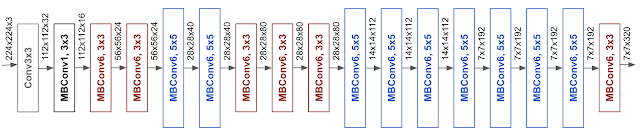
\includegraphics[width=\linewidth]{images/efficientnet.png}
  \caption{The architecture for EfficientNet's baseline network EfficientNet-B0 from \cite{2019arXiv190511946T}}
  \label{fig:efficientnet}
\end{figure}

Amazon has two AutoML products to offer - Amazon SageMaker Autopilot for the creation of the classification and regression machine learning models and Amazon DeepAR for forecasting scalar (one-dimensional) time series using RNN. This paper is also heavily based on the probabilistic approach used in DeepAR because of it’s spectacular results (see \ref{fig:deepar}).

\begin{figure}[]
  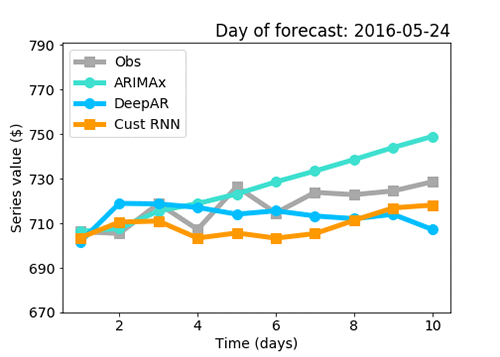
\includegraphics[width=\linewidth]{images/deepAr.png}
  \caption{Benchmark analysis: Visualization of forecasts produced by the RNN combo, ARIMAx and DeepAR together with what was actually observed for the series A values}
  \label{fig:deepar}
\end{figure}

This section would not be full without the paper which shares a lot in common with this project. RL agent (Q-Learning, epsilon-greedy exploration rate control, finite state space) described in the paper outperformed meta-modeling approaches for network design on image classification tasks \cite{Baker2016DesigningNN}.

The interest to the topic becomes even hotter when the NAS benchmark and dataset was introduced by Google Research team \cite{pmlr-v97-ying19a}

A variety of methods have been proposed to perform NAS, including reinforcement learning, Bayesian optimization with a Gaussian process model, sequential model-based optimization (SMAC), evolutionary search, and gradient descent over the past few years. We see a lot of research potential in this field and we share a big passion for RL paradigm - and that's why this project exists.

\section{Reinforcement Learning}

RL is a machine learning paradigm often used when the exact mathematical model is unknown and data is unlabeled. In this project, we would mainly concentrate on the Q Learning approach. We require having an observable environment where software agent would be able to take actions which would lead to reward. An agent is designed in the way it should maximize reward by utilizing existing knowledge (exploitation) or exploring random actions (exploration). The algorithm needs to learn a policy that determines which action should be taken next given current state (or set of recent states). The environment agent is operating with is typically a Markov Decision Process.

\subsection{Markov Decision Process}

MDP is a generalization of the mathematical framework which allows performing a sequence of actions in an environment where future states would depend on current states and yield partly random outcomes.

It is described by:
\begin{itemize}
  \item State (or states) $\sset$ that are fully observable by agent
  \item Set of actions $\aset$ which agent could take in a given state
  \item Transition model $\Tdef$ - an effect in the state accused by action taken by the agent
  \item A reward function $\Rfun$ which defines a reward received by an agent for taking this action
  \item A discount factor $\Ddef$ which is used to value a reward that could be received in future
  \item A policy $\pdef$ agent should learn
\end{itemize}

A policy that allows the agent to maximize its reward is called a solution of given MDP. Notation of MDP used above is taken from \cite{Thomas15a}.

MDP that we will refer to later in this thesis, would have a Markov property because the reward received from action taken in the current state is not depended on previous states nor previous actions. In other words, we are talking about the Markov chain in this thesis.

\subsection{Exploration and exploitation dilemma}
To demonstrate exploration over exploitation problem we usually often refer to Multiarmed Bandit Problem.

The multiarmed bandit problem is MDP with stochastic reward. Imagine having N machines with reward probabilities $R_1 .. R_n$. Playing k-th bandit could result in the reward of 1 with a probability of $R_k$ or in reward 0 with a probability of $1 - R_k$. Real reward probabilities are unknown to the agent. Also, resources are limited, so, exploring them using the law of large numbers is inefficient and impossible in terms of this problem.

The goal of the agent playing multiarmed bandits is the maximization of cumulative reward.

Simply said, while playing a known action (performing exploitation) agent may miss a better option. This becomes a loss function of such algorithms - a regret player might have due to not selecting the optimal action. If the agent always plays random actions (exploration) it will be completely useless and would yield no good results with limited resources given.
In other words, to balance exploration and exploitation problem we would need to ensure that the agent is not overfitting to known actions but still uses gained knowledge. It often happens, that RL agents observes some \textbf{good} \textbf{enough} action and starts to use it constantly. This is not the way we generally want an RL algorithm to behave.
\subsection{Epsilon-greedy approach}
Epsilon-greedy approach to solving exploration over exploitation dilemma is based on the idea, where an agent would generally take best actions, but at some time iterations t, it would explore random actions. It often assumes that at the beginning of the training number of random actions would be bigger (to ensure that agent would be able to explore good actions at the very beginning) and later it would decay (to ensure that agent is actually playing best actions). An expected reward is often represented as a mean of previously received rewards when playing this action. 

\subsection{Upper-confidence bound}

UCB is another instrument to solve exploration over exploitation dilemma. The general approach is similar to the epsilon-greedy algorithm, however, UCB allows us to use unexplored actions in favor of actions which algorithm is very certain about being bad ones.

UCB measures the potential of action using the upper confidence bound of the reward value in such a way that a larger number of trials of certain action should give smaller bound. This also prevents the algorithm from overfitting.

In this work we would refer to Theorem 1 from \cite{Auer2002} using a simple UCB approach which allows receiving logarithmic regret uniformly and without any preliminary knowledge about the reward distributions.

\[
U(a) = Q(a) + \sqrt{\frac{2 log n_a}{N}}
\]

Where Q(a) is expected reward from action a (generally a mean of rewards received by playing that action), $n_a$ is the number of times this action was played and N is a total number of plays.
\subsection{Deep Q Learning}
While Q learning is an algorithm that allows the agent to learn an effective policy for maximizing cumulative reward in general MDP, deep Q learning is the same, model-free approach that uses Deep Neural Network to approximate the values of expected reward.

In recent years a lot of research is done in this field, even though Deep Q learning is treated as an unstable solution because a slight change in input can change outputs significantly.

However, this approach has a proven success story. This work is inspired by \cite{MnihKSGAWR13} which was one of the first successful approaches to use a deep neural network as a backend for reinforcement learning agent.

In general Deep Q learning algorithms stores experienced rewards in replay memory, from where they are later batched and used as input to the underlying neural network.

This work uses a convolutional neural network as a backend for RL algorithm.
\section{Image classification problem}

The image classification problem is a machine learning problem aiming to recognize a visual concept of a given image and assign some class (label) to it as an output.

A data-driven approach for this problem required to train the algorithm on loads of images in order to understand which features images from one class have in common to other images of this class and different from images of other classes.

Naturally, in the beginning, KNN (K Nearest Neighbors) and other simple clusterization algorithms were used.

However, the real move forward started when backpropagation techniques were applied to neural network architectures, which opened a way for deep learning techniques. As Yann LeCun released LeNet-5  (see \cite{lecun-89c}) modern convolutional architectures started to develop rapidly.

There are several popular datasets such as MNIST [\cite{mnist}], Flowers [\cite{flowers}], ImageNet [\cite{imagenet}] etc. which are constantly used in image classification contests. Modern deep neural networks outperform human-level accuracy on those datasets.

\section{Convolutional Neural Networks}

CNN or ConvNet are neural networks sharing architecture of multi-layer perceptrons. Since multi-layer perceptrons have fully-connected layers, they are expensive in terms of computation resources. CNN shares a different approach - every convolutional neuron processes data only related to its receptive field of small size. Most ConvNets use fully connected layers at the end anyway.

Though CNN is capable of efficiently handling a huge variety of machine learning tasks, the simplest for understanding would be an image recognition example - and this is also related to the CNN architectures generated by the algorithm introduced by this project. One of the most popular ConvNet was LeNet-5. Figure \ref{fig:lenet} shows architecture of LeNet-5. 

\begin{figure}[!htb]
  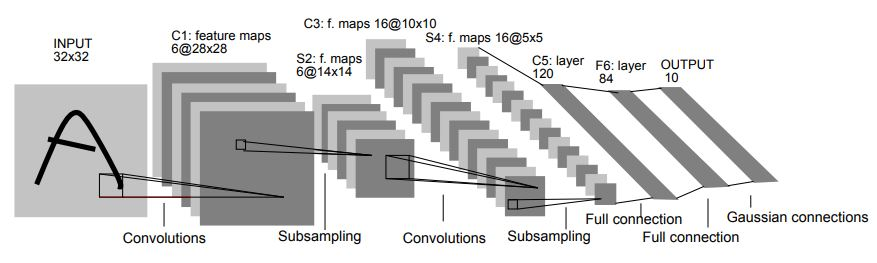
\includegraphics[width=\linewidth]{images/lenetoriginal.jpg}
  \caption{Original image from \cite{lecun-89c} displaying LeNet-5 architecture}
  \label{fig:lenet}
\end{figure}

Each neuron in a CNN computes an output applying a function over input values received from the receptive field (a small subset of input) in the previous layer. This function is usually a dot product over a matrix of weights. Bias also could be applied (matrix addition operation).

The learning process is performed by updating weight and bias matrices. Huge progress was gained after the backpropagation technique was introduced for modern deep neural networks [\cite{lecun-98b} - this is not an invention of the technique; it was introduced by lots of people before Yann LeCun, but this paper is a very good explanation of basic principles]. Backpropagation is a way to efficiently compute the gradient of the loss function with respect to the weights of the network.

\section{Gaussian Distribution and MLE }

Gaussian distribution or normal distribution is a continuous probability distribution of a random variable. This distribution is described by its mean and standard deviation.

The density curve is symmetrical and centered above its mean. It's spread is by the standard deviation.

Density curve is defined by following function:

\[
f(x) = \frac{1}{\sigma \sqrt{2 \pi}} e^{\frac{-1}{2}(\frac{x - \mu}{\sigma})^2}
\]

We would use the maximum likelihood estimate of the variance of the distribution $\sigma^2$ as a loss function of master CNN.

We want to estimate the parameters of distribution by maximizing a likelihood function so that observable data is most probable.

It is convenient to work with a log-likelihood interpretation

Let $l$ be a likelihood function (probability of observing the given data as a function of $\sigma$) and $f$ be a density function noted above.

\[
	l(\sigma, \mu) = \sum_{i=1}^{n}log(f(x_i | \sigma, \mu))
\]

Calculation of partial derivatives and setting them to zero gives MLE of the target variable (in our case - $\sigma$).
 
%\chapter{Proposed approach}

\section{Pipeline}
\section{RL agent}
\subsection{Reward function}
\subsection{Exploration and exploitation}
\subsection{Gaussian layer}
When it comes to probabilistic approach to RL algorithms, scoring becomes very important and may have a big impact on action taken by the controller - \cite[see][]{tilmann}

If master CNN in RL agent is solving a regression problem (which is exactly our case) this CNN would use backpropagation to update it's weights (as noted above) in a way that error metrics of a test set would be minimized. Originally outputs of the last layer would be simple values - in our case, values which determines the actions that would be taken by controller.

Those values obviously depends on input and weights. In order to receive a Gaussian distribution we would need to modify last layer so that it would return mean and variance of output variable, which is enough to describe a Gaussian distribution of this variable. This allows us to bring a prediction uncertainity into the outputs of CNN. As described in \cite{2017arXiv170404110S} this requires also another approach to computation of loss function.

Generally saying we are using Gaussian distribution instead of single values because we need to have a measure of uncertainity of prediction of output. Then, if we have quite big uncertainity, it would be smarter to explore a random action. Otherwise, agent should use predicted action.







\section{Master CNN}
\section{Slave CNN}

%\chapter{Experiments}

\section{Datasets}
\section{Metrics}
\section{Environment and training}
\section{Results}
 
%\chapter{Conclusion}

 

%----------------------------------------------------------------------------------------
%	THESIS CONTENT - APPENDICES
%----------------------------------------------------------------------------------------

\appendix % Cue to tell LaTeX that the following "chapters" are Appendices

% Include the appendices of the thesis as separate files from the Appendices folder
% Uncomment the lines as you write the Appendices


\chapter{Appendix A}

\section{Reproducibility and random seed}

Something on the topic



\endinput
%\include{Appendices/AppendixB}
%\include{Appendices/AppendixC}

%----------------------------------------------------------------------------------------
%	BIBLIOGRAPHY
%----------------------------------------------------------------------------------------

\printbibliography[heading=bibintoc]

%----------------------------------------------------------------------------------------

\end{document}  
